\documentclass[11pt]{article}
\usepackage[margin=1in]{geometry}
\usepackage[T1]{fontenc}
\usepackage{lmodern}
\usepackage{booktabs}
\usepackage{graphicx}
\usepackage{amsmath}
\usepackage{xcolor}
\usepackage{tikz}
\usepackage{caption}
\usepackage{hyperref}
\usepackage{url}
\hypersetup{colorlinks=true,linkcolor=blue!50!black,citecolor=blue!50!black,urlcolor=blue!50!black}

% Figures generated from the prompts in paper/prompt/ are optional: until the PNG exists,
% a framed placeholder naming the missing file is printed instead.
\newcommand{\maybefigure}[2]{%
  \IfFileExists{#1}{\includegraphics[width=#2]{#1}}{%
    \fbox{\parbox[c][4cm][c]{0.9#2}{\centering\small Figure pending: \texttt{\detokenize{#1}}\\(prompt in \texttt{paper/prompt/})}}}}

\definecolor{lorac}{HTML}{8DA0CB}
\definecolor{ftc}{HTML}{A6D854}
\definecolor{vlhc}{HTML}{FC8D62}
\definecolor{mixc}{HTML}{E78AC3}
\definecolor{ensc}{HTML}{B3B3B3}

\title{Adapting Apertus 1.5 for Product Image Classification:\\From Zero-Shot Prompting to a Fused Multi-Encoder Classifier}
% TODO: confirm the author list with the team before submission.
\author{Team BYMO}
\date{28 November 2026}
\begin{document}
\maketitle

\begin{abstract}
We adapt Apertus 1.5, a language model with a native vector-quantised (VQ) image tokenizer, to classify Galaxus product images along six dimensions. With zero-shot prompting, the best we reached on our coverage set was 0.583 macro F1 (70B), so we trained the 8B model on the task. After some exploratory micro-training we followed three directions: decoder fine-tuning, LoRA with classification heads, and LoRA with heads plus a SigLIP~2 visual adapter. The first two score 0.805 and 0.796 on the public development leaderboard. The visual adapter reaches 0.832 after we add OCR, spatial features, two-dimensional attention pooling and more data. Further variants (synthetic text overlays, a larger encoder, all labelled data, a trainable encoder) moved public dev by only $-0.003$ to $+0.0035$. In a third phase we fused frozen DINOv3 features into the SigLIP stream through a zero-initialised residual. This single-decoder model scores 0.842 on public dev; a two-model ensemble reaches 0.847. We deliver the single-decoder model. With merged LoRA, TF32 and selective perspective test-time augmentation, its inference path runs at 11.7 images/s on one H200, or about 2.4 GPU-hours per 100,000 images. The rarest classes have only 21 to 60 labelled examples in the whole dataset. We therefore pair a fixed, product-disjoint local split, whose resolution we quantify by bootstrap, with the public leaderboard, which decides between models. Training sets, schedules and auxiliary inputs changed together from run to run, so the results describe an engineering trajectory and should not be read as controlled ablations.
\end{abstract}

\section{Introduction}
Product catalog images have to be described consistently, whatever their viewpoint, background, packaging or visible text. We study a six-output classification task with Apertus 1.5 and try to balance predictive quality against the cost of adapting and serving an 8B-parameter model. The work went through several stages (Figure~\ref{fig:scores}), and each was motivated by what the previous one showed. We started from the data: an exploration of the dataset fixed how we train and how we measure (Section~\ref{sec:data}). A zero-shot benchmark of the 8B and 70B models then told us whether training was needed at all (Section~\ref{sec:zero}), and three exploratory micro-training phases chose the training formulation (Section~\ref{sec:micro}). Full training followed in three phases. In the first we ran three adaptation strategies in parallel (Section~\ref{sec:three}). In the second we added spatial readouts and extended the strongest strategy (Section~\ref{sec:phase2}), and in the third we fused a second image encoder into it (Section~\ref{sec:phase3}). Section~\ref{sec:inference} describes the optimised inference path. Some problems come back throughout the paper: rare classes, left/right perspective, small text, and how far comparisons across evaluation splits can be trusted.

In this paper we contribute (i) a dataset exploration whose findings are tied to the design and evaluation choices that follow; (ii) a quantified zero-shot baseline that shows how strongly prompt design affects Apertus on this task; (iii) a classification-head formulation that keeps Apertus' native VQ tokens and adds continuous SigLIP~2 and DINOv3 features through a shared set of 49 soft tokens; (iv) spatial readouts that address the mirror symmetry of mean-pooled features; (v) an inference path that nearly doubles the throughput of our original export (11.7 against 6.0 images/s on dev, and 14.3 without test-time augmentation on an H100), with a measured effect on predictions; and (vi) an evaluation protocol for a dataset whose rarest classes have a few dozen examples, with its resolution quantified.

\begin{figure}[t]
\centering
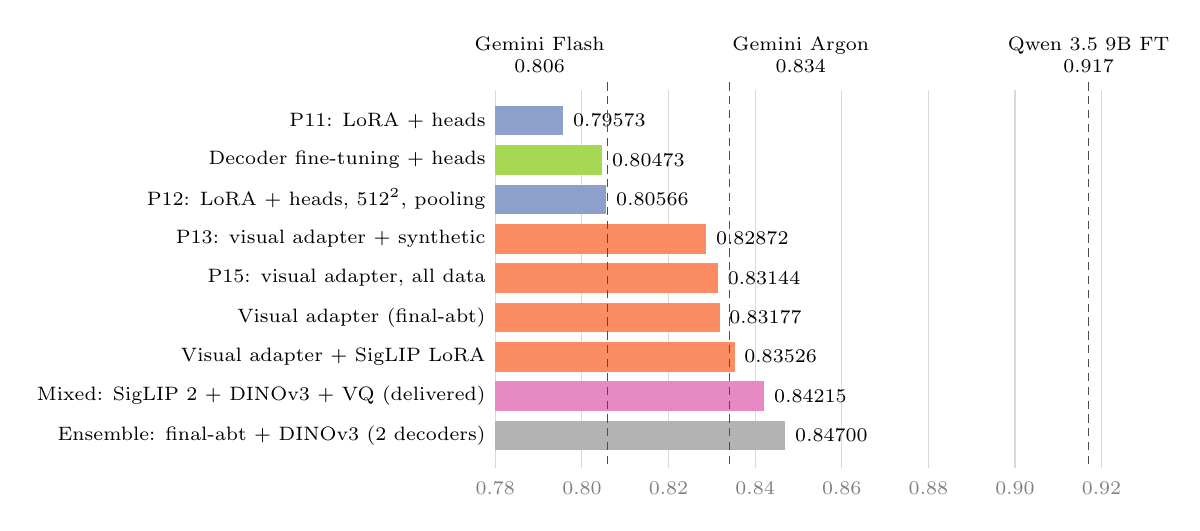
\begin{tikzpicture}[x=1cm,y=0.5cm]
  \foreach \t in {0.78,0.80,0.82,0.84,0.86,0.88,0.90,0.92} {
    \pgfmathsetmacro{\tx}{(\t-0.78)*55}
    \draw[gray!30] (\tx,0.4) -- (\tx,-9.2);
    \node[font=\scriptsize,gray] at (\tx,-9.7) {\t};
  }
  \foreach \i/\name/\v/\c in {
    0/{P11: LoRA + heads}/0.79573/lorac,
    1/{Decoder fine-tuning + heads}/0.80473/ftc,
    2/{P12: LoRA + heads, 512\textsuperscript{2}, pooling}/0.80566/lorac,
    3/{P13: visual adapter + synthetic}/0.82872/vlhc,
    4/{P15: visual adapter, all data}/0.83144/vlhc,
    5/{Visual adapter (final-abt)}/0.83177/vlhc,
    6/{Visual adapter + SigLIP LoRA}/0.83526/vlhc,
    7/{Mixed: SigLIP 2 + DINOv3 + VQ (delivered)}/0.84215/mixc,
    8/{Ensemble: final-abt + DINOv3 (2 decoders)}/0.84700/ensc} {
    \pgfmathsetmacro{\w}{(\v-0.78)*55}
    \fill[\c] (0,-\i) rectangle (\w,-\i-0.75);
    \node[left,font=\scriptsize] at (0,-\i-0.37) {\name};
    \node[right,font=\scriptsize] at (\w,-\i-0.37) {\v};
  }
  \foreach \b/\lbl/\anc in {0.806/{Gemini Flash}/south east,0.834/{Gemini Argon}/south west,0.917/{Qwen 3.5 9B FT}/south} {
    \pgfmathsetmacro{\bx}{(\b-0.78)*55}
    \draw[densely dashed,black!70] (\bx,0.6) -- (\bx,-9.2);
    \node[font=\scriptsize,anchor=\anc,align=center,inner xsep=1pt] at (\bx,0.6) {\lbl\\\b};
  }
\end{tikzpicture}
\caption{Public development leaderboard macro F1 of our submitted models, in increasing order, against the organiser baselines (dashed). Colours mark the model family: LoRA + heads (blue), decoder fine-tuning (green), SigLIP~2 visual adapter (orange), mixed SigLIP~2 + DINOv3 model (pink) and a two-decoder ensemble (grey). Each bar is a single submission without an uncertainty estimate.}
\label{fig:scores}
\end{figure}

\section{Dataset exploration}
\label{sec:data}
Before choosing a model we looked at what the data allow us to learn and to measure. This section reports what we found and the decision each finding led to; Table~\ref{tab:findings} collects the links to the later sections.

\subsection{Data and metric}
The challenge dataset comprises 22,429 images from 14,118 products: 11,876 labelled training images, 5,261 public development images and 5,292 final images. Train, dev and final share no product. The six dimensions are subject, background, perspective, individuals, text classification and text language, with 41 classes in total \cite{challenge}. Each label cell is either set or confirmed by a human, or an unchecked model prelabel, and a relevance flag marks cells where the dimension has no meaning. The official metric evaluates relevant human-labelled cells, computes class-macro F1 within each dimension and averages the six dimensions. The classes of a dimension are all classes in the labels \emph{plus every valid class a model predicts}, so a false positive on an absent rare class adds a class with zero F1. The organisers provide three reference scores on public dev: a fine-tuned Qwen 3.5 9B (0.917), Gemini 4 Argon (0.834) and Gemini 3.8 Flash (0.806). Only Apertus and open-weights supporting models may run at inference time \cite{challenge}.

\subsection{Findings and the decisions they drove}
The first four findings come from our initial exploration and shaped the design. The last four come from analyses we ran later to test the choices that the first ones had motivated; we report them here because they describe the data.

\paragraph{F1: the rarest classes are rare in the whole dataset.} \texttt{train.csv} holds only 21 human-labelled Dutch cells, 47 Italian and 60 certification seals (Table~\ref{tab:rare}). In the 9,344-image split of our first LoRA run, subject ranges from 5,210 full-product examples to 69 product groupings. Because macro F1 weights every class equally, these few examples carry as much weight as thousands of common ones. \emph{Decisions:} rare-class repetition and class-balanced focal loss, which we tested rather than assumed (Section~\ref{sec:micro}); synthetic overlays for the rarest text classes (Section~\ref{sec:extend}); a coverage set enriched with rare classes for method comparison; and the evaluation protocol of Section~\ref{sec:protocol}.

\begin{table}[ht]
\centering
\caption{The rarest classes (human, relevant cells). A larger holdout adds few rare examples to evaluation and takes them from training.}
\resizebox{\textwidth}{!}{\begin{tabular}{lrrrr}\toprule
Class & train.csv & Prompt-test & Left for training & 20\% holdout: test / training \\\midrule
Text language: Dutch & 21 & 4 & 17 & 4 / 17 \\
Text language: Italian & 47 & 4 & 43 & 9 / 38 \\
Text classification: certification seal & 60 & 6 & 54 & 12 / 48 \\
Subject: product grouping & 91 & 10 & 81 & 18 / 73 \\
Text language: other & 110 & 10 & 100 & 22 / 88 \\\bottomrule
\end{tabular}}
\label{tab:rare}
\end{table}

\paragraph{F2: part of the labels are unchecked prelabels.} About a fifth of the label cells are model prelabels, mostly where a dimension is not relevant. Among relevant cells the share of human labels exceeds 99.7\% everywhere except text language, where it is 59\%. \emph{Decision:} every loss and every local score uses only human, relevant cells, exactly as the leaderboard does; local scores use the official metric implementation.

\paragraph{F3: images come in product groups.} Products have 1.64 labelled images on average, and the same photo occasionally appears for two products. \emph{Decision:} all our splits are product-disjoint, derived from a hash of the product identifier so that every machine reproduces them without sharing image identifiers.

\paragraph{F4: image formats and the token budget.} Images reach 2,048 pixels on the longest side, about 4\% are PNGs with a transparent background (labelled as white), and a few are tiny, down to $1\times1$ pixel. Apertus' VQ tokenizer turns a 256-pixel square into 256 tokens and a 512-pixel square into 1,024 (Section~\ref{sec:apertus}). \emph{Decisions:} transparent images are composited on white; an unreadable image is replaced by a blank one so that every row gets a prediction; image resolution is treated as an explicit speed--accuracy trade-off (Section~\ref{sec:pooling}); and small text is read by OCR on the full-resolution image instead of relying on the VQ grid alone (Section~\ref{sec:extend}).

\paragraph{F5: a local split has limited resolution.} With a product-level bootstrap (2,000 resamples) on our 1,193-image test split, the delivered model scores 0.843 with a 95\% interval of [0.816, 0.864], and the per-class intervals of classes with four to six examples span most of [0, 1]. Paired differences between related checkpoints are resolved down to about 0.016, and between less similar models to about 0.03. \emph{Decision:} the two-signal protocol of Section~\ref{sec:protocol}.

\paragraph{F6: train and dev look alike.} The category mix of train and dev is nearly identical (total-variation distance 0.026), and only 0.3\% of dev images belong to a product type absent from training. \emph{Consequence:} a local split with the natural class distribution is a fair proxy for the leaderboard, and differences between local and public scores are better explained by F5 than by a distribution shift.

\paragraph{F7: the product context alone carries some signal.} A class-balanced logistic regression on word n-grams of title, type, brand, category and subcategory reaches 0.438 macro F1 on prompt-test, against 0.187 for the majority class and 0.376 for the majority class of each product type (Figure~\ref{fig:context}). It is strongest on text language (0.518, mostly from the language of the title). \emph{Consequence:} the context is worth giving to the model, and all our models receive it in the prompt; but it leaves a large gap that only the image and the text inside it can close.

\begin{figure}[ht]
\centering
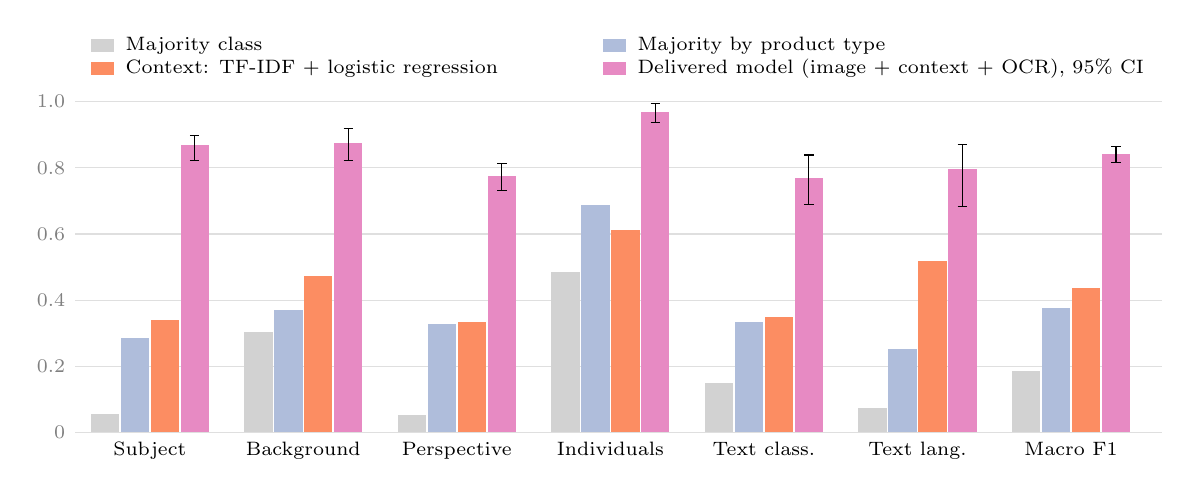
\begin{tikzpicture}[x=1cm,y=4.2cm]
  \foreach \t in {0,0.2,0.4,0.6,0.8,1.0} {
    \draw[gray!25] (-0.2,\t) -- (13.6,\t);
    \node[font=\scriptsize,gray,left] at (-0.2,\t) {\t};
  }
  \foreach \d/\name in {0/Subject,1/Background,2/Perspective,3/Individuals,4/Text class.,5/Text lang.,6/Macro F1} {
    \node[font=\scriptsize,below] at (\d*1.95+0.75,0) {\name};
  }
  \foreach \d/\a/\b/\c/\m/\lo/\hi in {
    0/0.056/0.285/0.340/0.868/0.821/0.899, 1/0.305/0.370/0.474/0.875/0.823/0.918,
    2/0.053/0.329/0.335/0.776/0.731/0.813, 3/0.486/0.689/0.613/0.970/0.936/0.994,
    4/0.150/0.333/0.349/0.769/0.688/0.839, 5/0.075/0.251/0.518/0.798/0.684/0.871,
    6/0.187/0.376/0.438/0.843/0.816/0.864} {
    \pgfmathsetmacro{\x}{\d*1.95}
    \fill[gray!35] (\x,0) rectangle (\x+0.36,\a);
    \fill[lorac!70] (\x+0.38,0) rectangle (\x+0.74,\b);
    \fill[vlhc] (\x+0.76,0) rectangle (\x+1.12,\c);
    \fill[mixc] (\x+1.14,0) rectangle (\x+1.50,\m);
    \draw[black] (\x+1.32,\lo) -- (\x+1.32,\hi);
    \draw[black] (\x+1.26,\lo) -- (\x+1.38,\lo); \draw[black] (\x+1.26,\hi) -- (\x+1.38,\hi);
  }
  \foreach \x/\y/\c/\l in {0/1.17/gray!35/{Majority class},6.5/1.17/lorac!70/{Majority by product type},0/1.10/vlhc/{Context: TF-IDF + logistic regression},6.5/1.10/mixc/{Delivered model (image + context + OCR), 95\% CI}} {
    \fill[\c] (\x,\y-0.02) rectangle (\x+0.3,\y+0.02);
    \node[font=\scriptsize,right] at (\x+0.32,\y) {\l};
  }
\end{tikzpicture}
\caption{F7: what the product context predicts on its own, against the delivered model, on prompt-test (macro F1 per dimension). Error bars are product-bootstrap 95\% intervals of the delivered model. The context helps most on text language and through product-type priors; every dimension needs the image.}
\label{fig:context}
\end{figure}

\paragraph{F8: images of one product share some labels, not all.} Among products with at least two scored images, all images share the label for 86\% of products on individuals, 74\% on background and 71\% on text classification, but only 63\% on text language, 41\% on subject and 20\% on perspective: a product's images deliberately show different views. Even a vote that uses the true labels of the sibling images gets 7--14\% of images wrong on individuals, background and text classification, 24\% on text language and 66\% on perspective. \emph{Consequence:} a product-level vote could at most break ties; we classify each image on its own.

\begin{table}[ht]
\centering
\caption{Findings from the dataset exploration and where they shape the work.}
\resizebox{\textwidth}{!}{\begin{tabular}{lll}\toprule
Finding & Decision & Section \\\midrule
F1 rare classes are rare in the whole dataset & repetition, class-balanced losses (tested), synthetic text, coverage set, protocol & \ref{sec:micro}, \ref{sec:extend}, \ref{sec:protocol} \\
F2 prelabels, 59\% human in text language & loss and scores on human, relevant cells only & all \\
F3 images in product groups & product-disjoint hashed splits & \ref{sec:protocol} \\
F4 large, transparent and tiny images; token budget & white compositing, blank fallback, resolution trade-off, OCR on full image & \ref{sec:pooling}, \ref{sec:extend} \\
F5 limited resolution of a local split (later analysis) & two signals: local split for diagnostics, public dev to decide & \ref{sec:protocol}, \ref{sec:extend} \\
F6 train and dev alike (later analysis) & natural-distribution local split as a proxy & \ref{sec:protocol} \\
F7 context alone reaches 0.438 (later analysis) & context in the prompt; the image is needed & \ref{sec:zero} \\
F8 labels partly shared within a product (later analysis) & per-image classification & -- \\\bottomrule
\end{tabular}}
\label{tab:findings}
\end{table}

\subsection{Evaluation protocol}
\label{sec:protocol}
Following F1, F3 and F6, our local sets come from hashing products into ten buckets. \emph{Prompt-test} (1,193 images of 713 products, 10\% of the training data) is one bucket and keeps the natural class distribution. \emph{Coverage} (2,532 images) adds a second bucket and 169 rare-class images, for comparing methods on rare classes. A balanced 450-image prototype set served the early micro-training only.

\paragraph{Why one fixed, product-level holdout.} F1 means that any holdout can contain only a handful of the rarest examples: prompt-test holds its proportional share, and doubling it to 20\% would add no Dutch example while removing Italian and seal examples from training, where they are scarcest. $K$-fold cross-validation would evaluate on every example, but it multiplies the cost of each experiment by $K$; our 8B training runs took one to three GPU-hours each, which put that out of reach in the time and budget of a hackathon. We therefore fixed one split that is product-disjoint, keeps the natural class distribution (a fair proxy by F6) and stays the same for every experiment, so that all comparisons are paired on identical images.

\paragraph{Two complementary signals.} Dev labels are hidden, so only prompt-test gives per-dimension and per-class diagnostics; the public leaderboard scores 5,261 images we never label or train on, but returns one overall number per submission. We used prompt-test to diagnose errors and to choose among checkpoints of a run, and public dev to decide between models. By F5, a gain below about 0.016 on prompt-test, or one carried by the rarest classes, counted as unconfirmed until public dev agreed. In the third phase prompt-test also chose the epoch within the run, because a separate validation set would have taken more rare examples away from training; it was a choice among five checkpoints of one run, and public dev confirmed it.

\section{Benchmark: can Apertus solve the task without training?}
\label{sec:zero}
The first decision was whether to spend our GPU budget on training at all. We therefore benchmarked Apertus as it comes, through prompting only.

\subsection{Apertus and its visual representation}
\label{sec:apertus}
Apertus 1.5 processes images through a VQ visual tokenizer that maps $16\times16$-pixel patches to discrete vocabulary tokens, which the language model reads alongside text tokens \cite{apertus} (Figure~\ref{fig:native}). The 8B model has 32 decoder layers. Because quantisation is an argmax, there is no gradient path from the decoder back into the image representation. For fine-grained product classification this leaves open whether discretisation and the resolution budget keep enough detail for small text and viewpoint; we treat it as a design hypothesis, not a demonstrated cause of our errors.

\begin{figure}[ht]
\centering
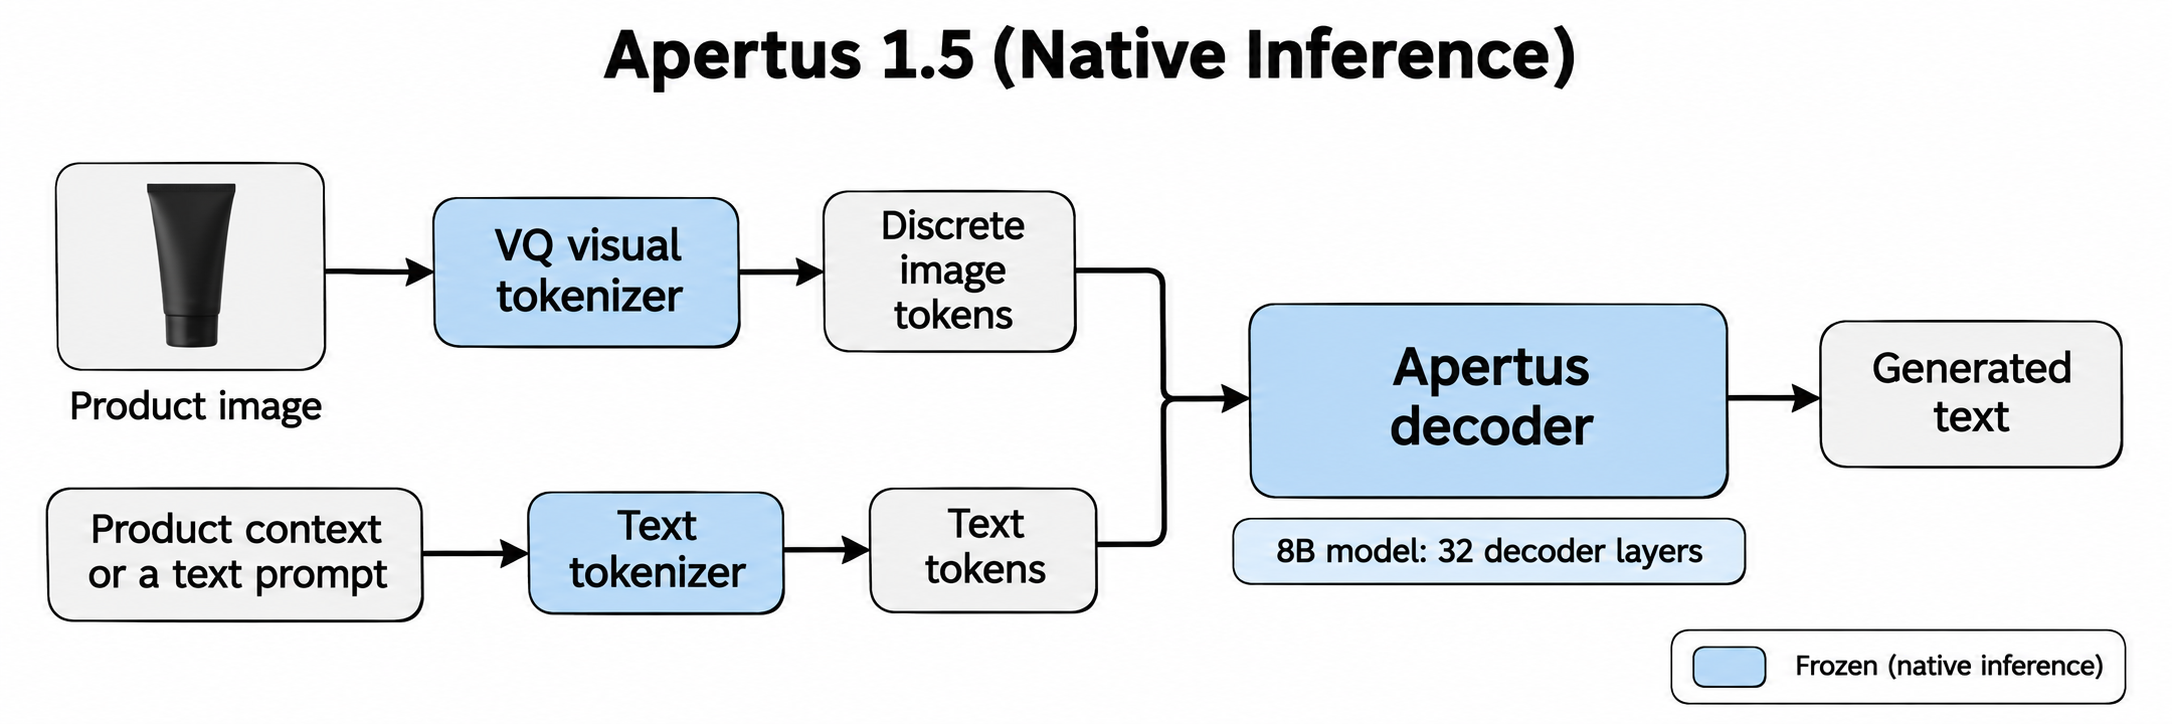
\includegraphics[width=0.85\textwidth]{figures/apertus-native.png}
\caption{Native Apertus 1.5 inference: the image passes through the frozen VQ tokenizer, the product context through the text tokenizer, and the decoder generates text.}
\label{fig:native}
\end{figure}

\subsection{Prompt design and zero-shot results}
We evaluated Apertus 1.5 8B and 70B through the hackathon's Keera API at 512-pixel resolution and temperature zero. Our early prompts asked for all six labels at once in JSON, with either brief or detailed instructions. On a balanced diagnostic sample, long rule-laden instructions pushed almost every subject prediction onto \texttt{full\_product} (subject macro F1 0.01 for 8B and 0.07 for 70B). When we replaced the rules with one line per class and asked for a free-text description first, subject macro F1 rose to 0.54 and 0.63. This became the \emph{v2} protocol, which sends seven sequential requests per image: one description, then six one-letter questions. We selected prompts on prompt-dev and checked them afterwards on prompt-test.

\begin{table}[ht]
\centering
\caption{Zero-shot macro F1. ``Minimal JSON'' is the early single-request prompt; ``rule-laden JSON'' is a long prompt with detailed labelling rules; v2 is the description-then-codes protocol. Throughput was measured on the shared gateway with 32 parallel requests.}
\begin{tabular}{llrrr}\toprule
Model & Prompt & Coverage (2,532) & Prompt-test (1,193) & Images/s \\\midrule
8B & Minimal JSON & 0.316 & 0.291 & -- \\
8B & Rule-laden JSON & 0.229 & 0.225 & 9.6 \\
70B & Rule-laden JSON & 0.304 & 0.294 & 4.1 \\
8B & Description + codes (v2) & 0.528 & 0.502 & 3.8 \\
70B & Description + codes (v2) & \textbf{0.583} & \textbf{0.590} & 2.8 \\\bottomrule
\end{tabular}
\label{tab:zero}
\end{table}

\begin{figure}[ht]
\centering
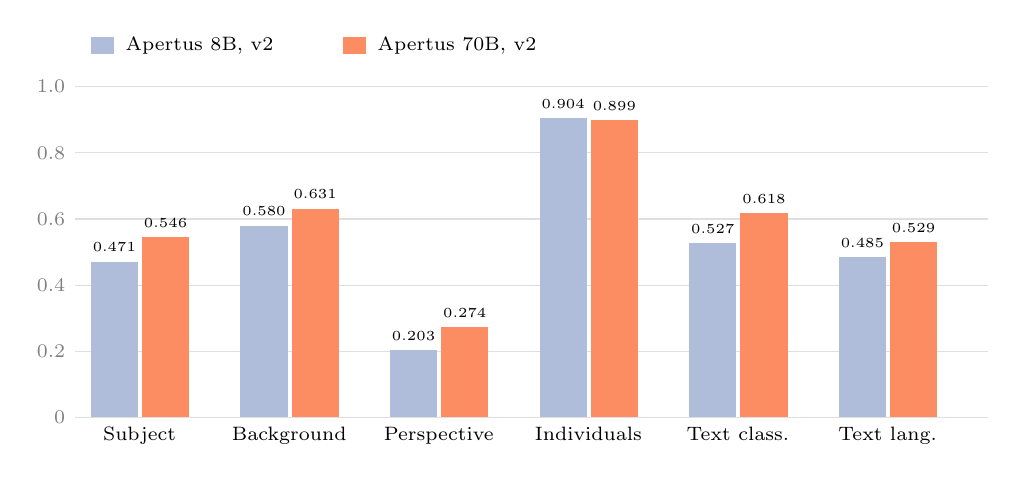
\begin{tikzpicture}[x=1cm,y=4.2cm]
  \foreach \t in {0,0.2,0.4,0.6,0.8,1.0} {
    \draw[gray!25] (-0.2,\t) -- (11.4,\t);
    \node[font=\scriptsize,gray,left] at (-0.2,\t) {\t};
  }
  \foreach \d/\name/\a/\b in {0/Subject/0.471/0.546,1/Background/0.580/0.631,2/Perspective/0.203/0.274,3/Individuals/0.904/0.899,4/Text class./0.527/0.618,5/Text lang./0.485/0.529} {
    \pgfmathsetmacro{\x}{\d*1.9}
    \fill[lorac!70] (\x,0) rectangle (\x+0.6,\a);
    \fill[vlhc] (\x+0.65,0) rectangle (\x+1.25,\b);
    \node[font=\tiny,above] at (\x+0.3,\a) {\a};
    \node[font=\tiny,above] at (\x+0.95,\b) {\b};
    \node[font=\scriptsize,below] at (\x+0.62,0) {\name};
  }
  \fill[lorac!70] (0,1.10) rectangle (0.3,1.15); \node[font=\scriptsize,right] at (0.32,1.125) {Apertus 8B, v2};
  \fill[vlhc] (3.2,1.10) rectangle (3.5,1.15); \node[font=\scriptsize,right] at (3.52,1.125) {Apertus 70B, v2};
\end{tikzpicture}
\caption{Zero-shot macro F1 per dimension on coverage with the v2 protocol. Perspective is the weakest dimension for both models.}
\label{fig:zeroshot}
\end{figure}

The prompt alone changes the score by more than a factor of two (Table~\ref{tab:zero}), and under v2 the 70B model beats 8B by 0.055 [0.041, 0.069] on coverage. Figure~\ref{fig:zeroshot} shows where both fail: perspective stays near 0.2--0.3, with zero F1 on \texttt{front\_angle\_left} and on both \texttt{back\_angle} classes for 70B. The v2 protocol is also slow, since it needs about 10,000 prompt tokens per image. Two comparisons settled the question. First, 8B v2 reaches 0.502 on prompt-test, only 0.064 above what the product context alone gives (F7), so zero-shot Apertus 8B extracts little from the image. Second, we considered distilling the 70B model, but even at confidence above 0.90 it is right on perspective only 63\% of the time, so it would be a poor teacher for our weakest dimension. \emph{Decision:} train the 8B model on the task, with perspective as a main target.

\section{Exploratory micro-training}
\label{sec:micro}
The benchmark said that we had to train; it did not say how. Before committing GPU budget to full runs, we ran three small experiments on a 1,500-image training split, evaluated on the balanced 450-image set, to answer three questions: which decoder layer carries the most useful features and whether a class-balanced loss pays off (F1); whether a generative formulation beats classification heads; and whether continuous image features can be injected next to the VQ tokens.

\subsection{Micro phase 1: classification heads on frozen Apertus}
We first trained six classification heads with a shared 512-unit hidden layer on frozen Apertus 8B representations of 512-pixel images. Each representation was the last-prompt-token state concatenated with the mean of the image-token states. We probed layers 12 to 32, and layer 24 gave the best internal-validation score (0.673 for cross-entropy); this is why we later truncated the decoder to its first 24 layers. On the balanced 450-image set, cross-entropy reached 0.542 macro F1 against 0.528 for focal loss \cite{focal} in a single-seed run, and a pixel-only baseline reached about 0.257. Over five seeds, strongly weighted cross-entropy averaged 0.557 and strongly weighted focal loss 0.547. Focal loss was a plausible answer to the imbalance of F1, but in these frozen-feature tests it did not beat cross-entropy, and GradNorm did not help either. \emph{Decisions:} truncate the decoder at layer 24, and keep the loss choice open per branch instead of adopting focal loss everywhere.

\subsection{Micro phase 2: generative LoRA}
A generative LoRA \cite{lora_paper} trained on 1,500 images reached 0.696 on the 450-image set and 0.734 on coverage, with a large advantage on perspective (0.484 against 0.230 for the heads). We cannot attribute the gap to LoRA alone, because the training set, resolution (256 against 512 pixels) and output format all differed from the frozen-head runs. \emph{Decision:} adapt the decoder (with LoRA or full fine-tuning) instead of freezing it, but keep classification heads, which give a probability for every class and cannot produce invalid outputs (the generative model produced 9 invalid answers on the 450-image set).

\subsection{Micro phase 3: a continuous visual adapter}
In parallel, we tested a frozen SigLIP~2 encoder \cite{siglip2} with a trainable two-layer projector that supplies 49 continuous image tokens to a frozen Apertus, alongside the native VQ tokens. This projector-only model still generated JSON. It obtained 0.467 and 0.516 on the 450-image set after the first and second epochs, but the second epoch also changed the batch size and restarted the optimiser. The experiment showed that continuous tokens can be injected next to VQ tokens. We did not compare it with a matched VQ-only model, so it does not show that the encoder adds information. \emph{Decision:} carry the adapter into full training as one of three directions.

\section{Training phase one: three directions}
\label{sec:three}
Full training went through three phases. Phase one compares three adaptation strategies, phase two improves them (Section~\ref{sec:phase2}) and phase three adds a second image encoder (Section~\ref{sec:phase3}). Figure~\ref{fig:architecture} shows the three strategies we pursued in parallel in phase one. In all of them, six classification heads read from decoder states take the place of text generation.

\begin{figure}[ht]
\centering
\IfFileExists{figures/three-strategies-revised.png}{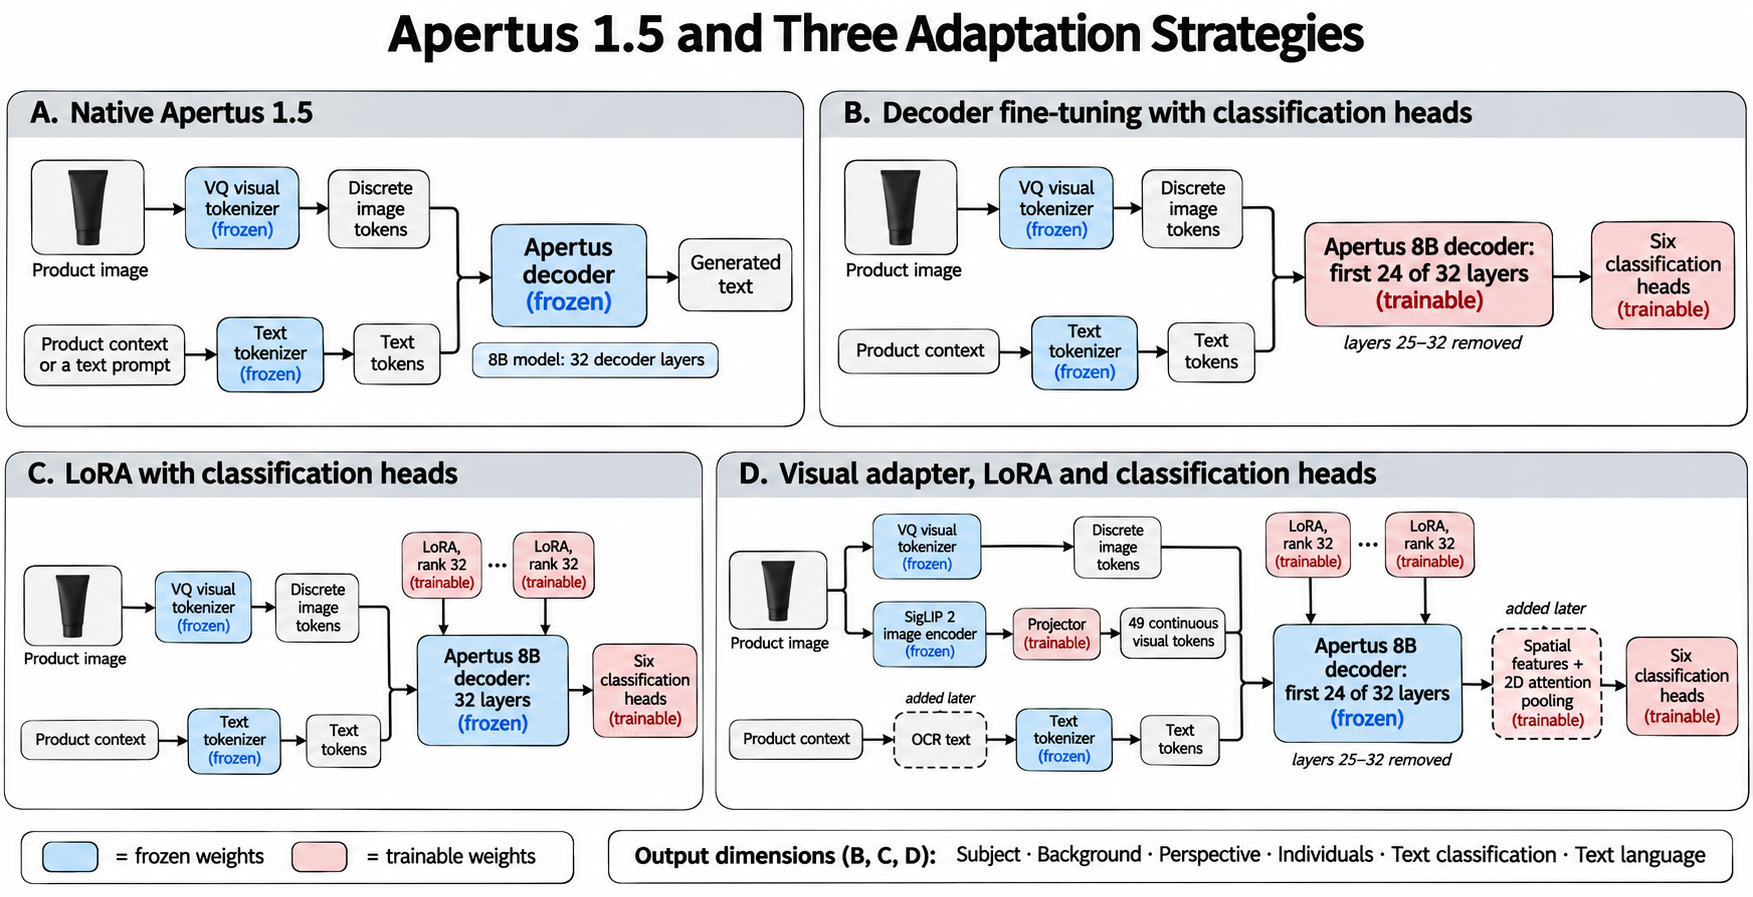
\includegraphics[width=\textwidth]{figures/three-strategies-revised.png}}{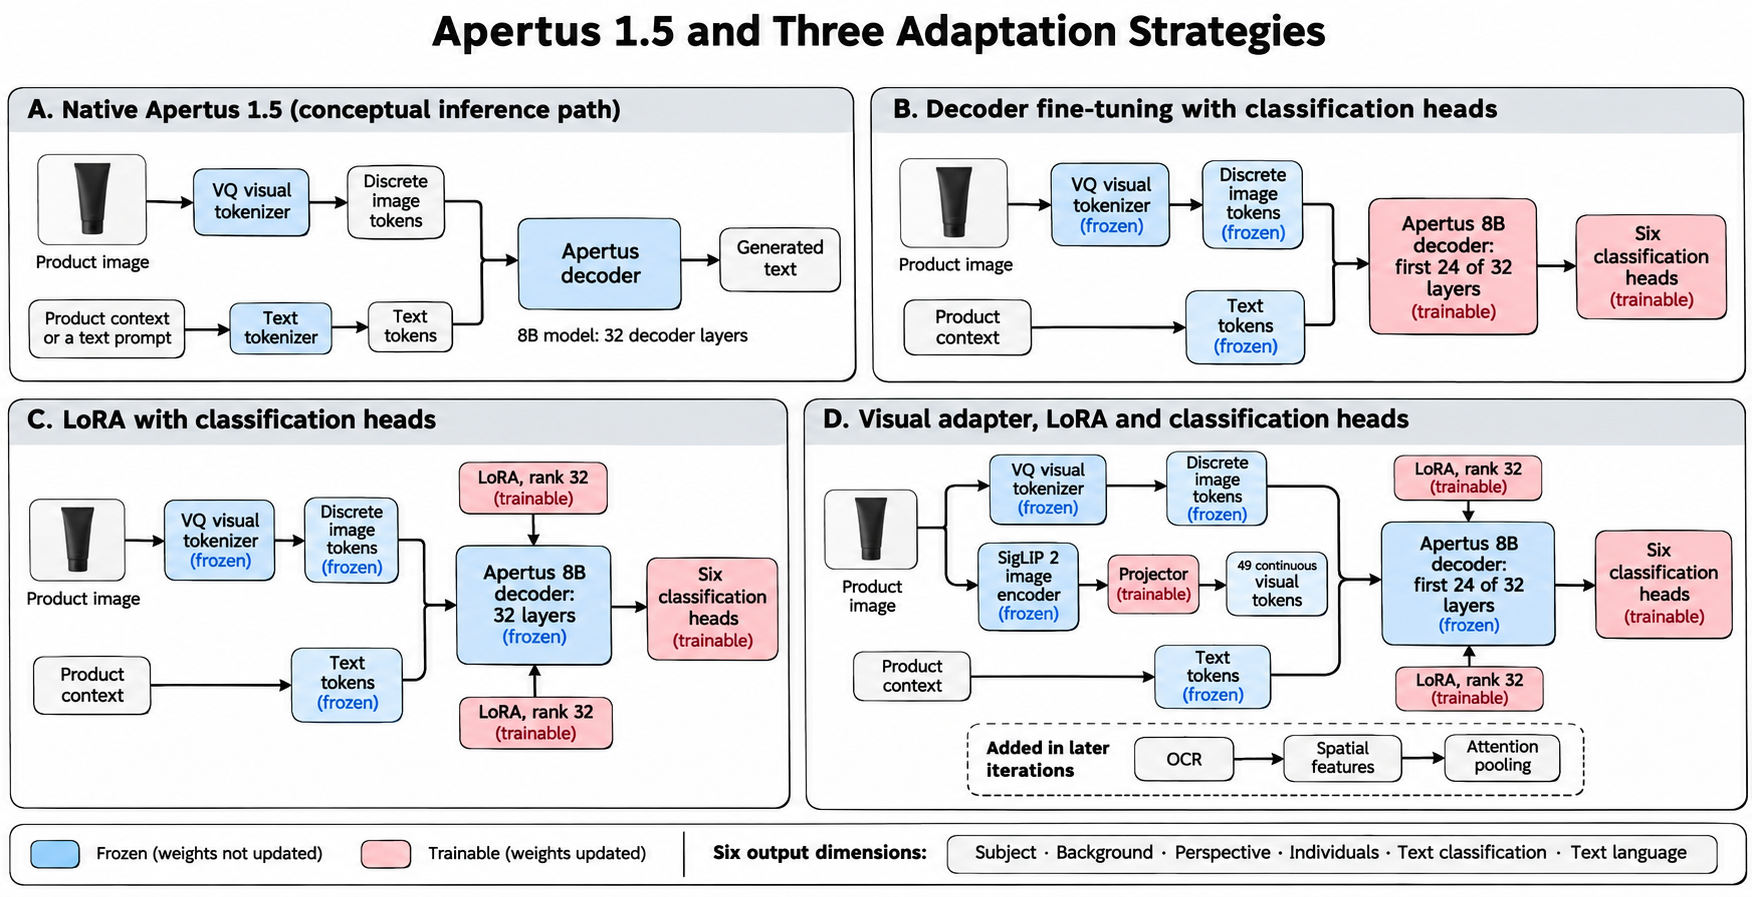
\includegraphics[width=\textwidth]{figures/apertus-training-phase-1.png}}
\caption{Native Apertus 1.5 (A) and the three phase-one adaptation strategies (B--D). Frozen and trainable labels apply to model weights, not token values. In B and D the decoder is truncated: layers 25--32 are removed, not frozen. Dashed boxes in D mark components added in phase two: OCR text, read from the product image, enters the prompt; spatial features and attention pooling act on decoder outputs before the heads.}
\label{fig:architecture}
\end{figure}

\emph{Decoder fine-tuning} truncates Apertus to its first 24 layers and trains those layers together with the heads, keeping the VQ tokenizer and embeddings frozen. The run trained about 5.24 billion parameters on all 11,876 labelled images with focal loss, class weights, rare-class repetition and mirroring. It took about 165 minutes on an A100 80~GB, with 57.1~GB peak memory.

\emph{LoRA with heads} jointly trained rank-32 LoRA adapters and six heads on the full 32-layer decoder. The initial P11 run used 9,344 training images (excluding all coverage products), 256-pixel inputs, three epochs, unweighted cross-entropy and about 83.9 million trainable parameters. It reached 0.781 macro F1 on coverage and 0.791 on prompt-test.

The \emph{visual adapter} combined frozen SigLIP~2, a trainable projector, native VQ tokens, rank-32 LoRA and six heads on the 24-layer decoder. Its first checkpoint, trained on 8,403 images, reached 0.742 on coverage and 0.750 on prompt-test, \emph{below} P11. Only the phase-two improvements made it the strongest branch (Section~\ref{sec:phase2}).

\begin{table}[ht]
\centering
\caption{The three directions. Public dev scores refer to different checkpoints and training configurations, not a controlled ablation. The final visual-adapter checkpoint (\emph{final-abt}) is a three-stage continuation of the first one.}
\resizebox{\textwidth}{!}{\begin{tabular}{llrrl}\toprule
Direction & Configuration & Training images & Public dev & Local evidence \\\midrule
Decoder fine-tuning & 24 layers + heads & 11,876 & 0.805 & No held-out coverage score \\
LoRA + heads (P11) & 32 layers, 256\textsuperscript{2} & 9,344 & 0.796 & Coverage 0.781; prompt-test 0.791 \\
Visual adapter, first checkpoint & 24 layers, SigLIP~2 + VQ & 8,403 & -- & Coverage 0.742; prompt-test 0.750 \\
Visual adapter, final-abt & + OCR, spatial features, pooling & 8,403 $\rightarrow$ 9,645 & 0.832 & Prompt-test 0.821 \\\bottomrule
\end{tabular}}
\label{tab:three}
\end{table}
We used the comparison in Table~\ref{tab:three} to decide which direction to continue. It does not isolate the architecture, since training data, augmentation, supervision, decoder depth, resolution and auxiliary inputs all differ. Decoder fine-tuning used all labelled images and therefore has no valid held-out score. Because final-abt trained on the coverage products outside prompt-test, its coverage score is not valid either. Decoder fine-tuning is the fastest model at inference (14.6 images/s on an H200, against 13.3 for P11 and 6.9 for final-abt) but stores 10.5~GB of decoder weights instead of a few hundred megabytes of adapters.

\section{Training phase two: spatial readouts and extensions}
\label{sec:phase2}
The main error of phase one was left/right perspective. Phase two addresses it in both remaining branches and then extends the visual adapter with OCR, more data and further variants.

\subsection{Spatial information and pooling}
\label{sec:pooling}
All three branches mixed up left and right. P11, for example, confused \texttt{front\_angle\_left} and \texttt{front\_angle\_right} 136 times on coverage. The cause is structural. The mean of the image-token states is nearly identical for an image and its mirror, and Apertus encodes positions only through rotary embeddings, which a mean discards. With mean features, the visual adapter chose the correct side only 55\% of the time, and 92\% of its left/right probabilities lay between 0.35 and 0.65.

We therefore added two readouts to the visual adapter, both through zero-initialised branches so that a resumed checkpoint is unchanged at step 0. \emph{Spatial features} are the differences between the mean states of the left and right halves and of the top and bottom halves of each image-token grid; they change sign under mirroring. \emph{Two-dimensional attention pooling} uses eight learned queries over all image tokens, with keys augmented by Fourier features of each token's row and column. In the training step that introduced them, prompt-test perspective rose from 0.54 to 0.76. The same step also added data and epochs, so we cannot credit the gain to the readouts alone.

We then ported the method to the LoRA-heads branch as P12, together with 512-pixel inputs and two epochs in place of three. Coverage macro F1 rose from 0.781 to 0.806 and public dev from 0.796 to 0.806, while prompt-test stayed at 0.791. On coverage, left/right swaps fell from 200 to 85 and perspective improved from 0.625 to 0.744, while subject and background declined slightly. Inference became 3.4 times slower (3.9 against 13.2 images/s), mostly because of the larger image. Resolution, pooling and training length changed together, and none of them can be credited on its own.

\subsection{Extending the visual adapter}
\label{sec:extend}
The visual adapter reached its final-abt checkpoint in three stages. Starting from the first checkpoint, an OCR stage added text read by docTR \cite{doctr} (a \texttt{fast\_base} detector and a multilingual PARSeq recogniser \cite{parseq}) on the original full-resolution image. The text, at most 300 characters with the largest text first, enters the prompt as a plain \texttt{<ocr>} block; there are no OCR-specific parameters. This stage did not raise overall prompt-test macro F1 (0.750 to 0.741) but improved German (0.79 to 0.86) and French (0.63 to 0.69) on coverage. It also added an epoch and halved the learning rates, so the effect is confounded. The third stage added spatial features and attention pooling, trained for three more epochs on all 9,645 images outside prompt-test and an internal validation set, and reached 0.821 on prompt-test and 0.832 on public dev. It has about 98 million trainable parameters. An early random-crop augmentation removed more than 1\% of the image content in 231 of 300 sampled crops (more than 5\% in 129), enough to turn some full-product views into close-ups. We replaced it with a label-preserving rescaling of the VQ input. The first checkpoint, and possibly the OCR stage, were trained with the old crops.

We then tested three continuations of final-abt and one encoder change (Figure~\ref{fig:lineage}, Table~\ref{tab:phase2}). For \emph{synthetic text} (P13) we generated 1,040 images from training products, adding promotional banners in under-represented languages (Dutch, Italian, other languages, French), generic seal-like badges and wordless icons. The generator labels the text dimensions, and the other dimensions keep the source image's labels. One extra epoch with 939 of these images raised prompt-test to 0.847 (+0.026, 95\% CI [0.004, 0.045]), and text language rose from 0.720 to 0.840. Public dev, however, fell slightly to 0.829. The prompt-test gain sat in classes with four to ten examples; without classes below ten examples it shrinks to about +0.010. With \emph{a larger encoder} (P14), SigLIP~2 so400m at 512 pixels pooled to 196 soft tokens with a new projector, the model reached 0.833 on prompt-test (+0.012, CI [$-0.001$, 0.027]) and had the best subject and text-classification scores. We did not score it on public dev, and it needed 80.7~GB at inference. The \emph{all data} run (P15) trained one more epoch on all 11,876 images and gave 0.831 on public dev, a tie with final-abt. Finally, we made the \emph{encoder trainable} with a rank-16 LoRA on SigLIP, trained together with the rest of the model for two epochs. This gave 0.835 on public dev (+0.0035).

\begin{figure}[ht]
\centering
\maybefigure{figures/phase2-lineage.png}{\textwidth}
\caption{Lineage of the phase-two checkpoints. The visual-adapter branch grows from its first checkpoint through an OCR stage to final-abt, which is the starting point of all later variants and of phase three. Spatial features and attention pooling were developed in this branch and later ported to LoRA + heads (P12).}
\label{fig:lineage}
\end{figure}

\begin{table}[ht]
\centering
\caption{Visual-adapter checkpoints on prompt-test (macro F1 per dimension) and public dev. P11 and P12 are LoRA-heads references. P15 trained on prompt-test and has no local score.}
\resizebox{\textwidth}{!}{\begin{tabular}{lrrrrrrrr}\toprule
Checkpoint & Macro F1 & Subject & Backgr. & Persp. & Indiv. & Text cl. & Text lang. & Public dev \\\midrule
P11 (LoRA + heads) & 0.791 & 0.861 & 0.894 & 0.620 & 0.990 & 0.805 & 0.577 & 0.796 \\
P12 (+ pooling, 512\textsuperscript{2}) & 0.791 & 0.832 & 0.872 & 0.752 & 0.969 & 0.736 & 0.588 & 0.806 \\\midrule
First checkpoint & 0.750 & 0.828 & 0.803 & 0.586 & 0.960 & 0.772 & 0.550 & -- \\
+ OCR & 0.741 & 0.816 & 0.808 & 0.544 & 0.955 & 0.771 & 0.554 & -- \\
final-abt (+ spatial, pooling, data) & 0.821 & 0.846 & 0.881 & 0.755 & 0.959 & 0.766 & 0.720 & 0.832 \\
P13 (+ synthetic text) & 0.847 & 0.845 & 0.870 & 0.783 & 0.965 & 0.780 & 0.840 & 0.829 \\
P14 (so400m, 512\textsuperscript{2}) & 0.833 & 0.868 & 0.886 & 0.768 & 0.965 & 0.805 & 0.707 & -- \\
SigLIP LoRA & 0.836 & 0.860 & 0.873 & 0.777 & 0.970 & 0.793 & 0.740 & 0.835 \\
P15 (all data) & -- & & & & & & & 0.831 \\\bottomrule
\end{tabular}}
\label{tab:phase2}
\end{table}

These variants are where the second signal of Section~\ref{sec:protocol} mattered. \emph{After final-abt, the gains we saw on prompt-test were not confirmed on public dev.} P13's +0.026 on prompt-test became $-0.003$ on dev, and the SigLIP LoRA's +0.014 became +0.0035. Both gains were concentrated in classes with four to ten prompt-test examples, where one prediction changes a class's recall by 0.10 to 0.25 and the per-class intervals span most of [0, 1]. Train and dev have nearly the same category mix, so a distribution shift does not explain the gap; the size of the rarest classes does. Synthetic overlays may also differ from real packaging text. By our rule these gains remain unconfirmed. None of the variants went into the delivered model, which builds on final-abt.

\begin{figure}[ht]
\centering
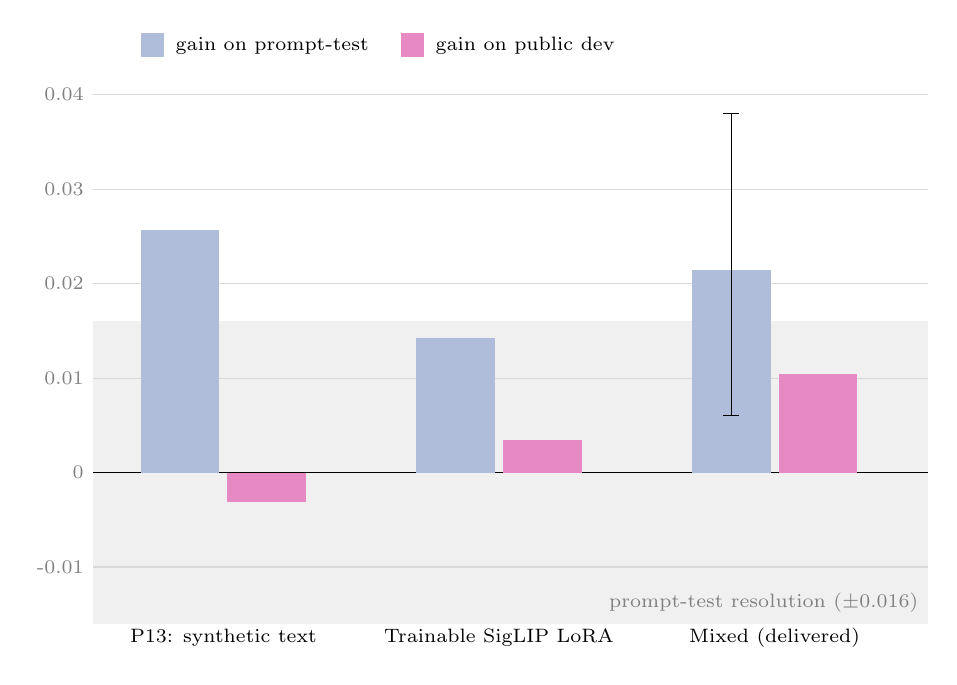
\begin{tikzpicture}[x=1cm,y=120cm]
  \fill[gray!12] (-0.3,-0.016) rectangle (10.3,0.016);
  \node[font=\scriptsize,gray,anchor=south east] at (10.3,-0.0158) {prompt-test resolution ($\pm$0.016)};
  \foreach \t in {-0.01,0,0.01,0.02,0.03,0.04} {
    \draw[gray!30] (-0.3,\t) -- (10.3,\t);
    \node[font=\scriptsize,gray,left] at (-0.3,\t) {\t};
  }
  \draw[black] (-0.3,0) -- (10.3,0);
  \foreach \x/\name/\p/\d in {0/{P13: synthetic text}/0.0257/-0.0031,3.5/{Trainable SigLIP LoRA}/0.0142/0.0035,7/{Mixed (delivered)}/0.0214/0.0104} {
    \fill[lorac!70] (\x+0.3,0) rectangle (\x+1.3,\p);
    \fill[mixc] (\x+1.4,0) rectangle (\x+2.4,\d);
    \node[font=\scriptsize] at (\x+1.35,-0.0175) {\name};
  }
  \draw[black] (7.8,0.006) -- (7.8,0.038); \draw[black] (7.7,0.006) -- (7.9,0.006); \draw[black] (7.7,0.038) -- (7.9,0.038);
  \fill[lorac!70] (0.3,0.044) rectangle (0.6,0.0465); \node[font=\scriptsize,right] at (0.62,0.0452) {gain on prompt-test};
  \fill[mixc] (3.6,0.044) rectangle (3.9,0.0465); \node[font=\scriptsize,right] at (3.92,0.0452) {gain on public dev};
\end{tikzpicture}
\caption{Gains over final-abt on the two signals of the protocol. P13 and the trainable SigLIP LoRA gain on prompt-test but not, or barely, on public dev; the delivered mixed model gains on both (paired 95\% interval on prompt-test shown as a bar). Two variants without both scores (P14, P15) are omitted.}
\label{fig:signals}
\end{figure}

\section{Training phase three: fusing DINOv3 into a single decoder}
\label{sec:phase3}
SigLIP~2 is trained to align images with text. We hypothesised that a self-supervised encoder trained on dense features, DINOv3 \cite{dinov3}, would add geometric information useful for perspective. A \emph{DINO-only} variant replaced SigLIP and the VQ tokens with 81 DINOv3 ViT-B/16 tokens (288-pixel padded input), warm-started LoRA, heads and pooling from final-abt, and trained with synthetic text. On prompt-test it was weaker overall than final-abt (0.808 against 0.821), much weaker on subject (0.772 against 0.846), but the best single model on perspective (0.783) and better on text language (0.781 against 0.720). The two encoders turned out to be complementary. A 50/50 probability ensemble of final-abt and DINO-only scored 0.850 on prompt-test and \textbf{0.847 on public dev}, our best leaderboard score, but it needs two decoders and therefore halves throughput.

\begin{figure}[ht]
\centering
\maybefigure{figures/mixed-architecture.png}{\textwidth}
\caption{The mixed model. DINOv3 features are pooled to the $7\times7$ SigLIP grid, passed through a zero-initialised LayerNorm--Linear layer and added to the SigLIP features before the existing projector, so the decoder still receives 49 soft tokens. Native VQ tokens, product context and OCR text complete the sequence for a single 24-layer Apertus decoder with LoRA; spatial features and attention pooling feed six classification heads.}
\label{fig:mixed}
\end{figure}

With the \emph{mixed} model we tried to keep what each encoder contributes to the ensemble while using a single decoder (Figure~\ref{fig:mixed}). DINOv3 runs at 288 pixels; its $18\times18$ patch grid is average-pooled to $7\times7$ and added to the pooled SigLIP features through a residual LayerNorm and $768\times768$ linear layer whose weight starts at zero. At step 0 the model therefore reproduces final-abt exactly. Before training, an assertion on the GPU checks this, along with a finite, non-zero gradient into the fusion layer. DINOv3 adds no tokens, so the decoder sequence is as long as final-abt's. The VQ tokenizer, both encoders, OCR and the Apertus base weights stay frozen; the fusion layer, projector, heads and decoder LoRA are trained, about 98.5 million parameters in total.

Training ran on one H200 on Modal from cached frozen features: 10,683 real images outside prompt-test, 521 rescaled views of rare text classes and all 1,040 synthetic images, whose loss is restricted to the two text dimensions and weighted 0.25. A half epoch trained only the fusion layer, then up to four joint epochs trained all trainable parts with AdamW (learning rates $6\times10^{-5}$ for fusion, $4\times10^{-5}$ for projector and heads, $1.5\times10^{-5}$ for LoRA) and focal loss with class-balanced weights \cite{cbloss}. We selected the checkpoint on prompt-test. Macro F1 there rose from 0.821 (step 0) to 0.829 after the fusion-only half epoch and to 0.843 after the third joint epoch. The fourth epoch lowered it to 0.837 while the training loss kept falling, so the third was selected. The hyperparameters above are those of the committed code at the time of training. The job took about two hours: 23 minutes to build the feature cache and about 18 minutes per joint epoch, with 61~GiB peak memory (Figure~\ref{fig:trajectory}).

\begin{figure}[ht]
\centering
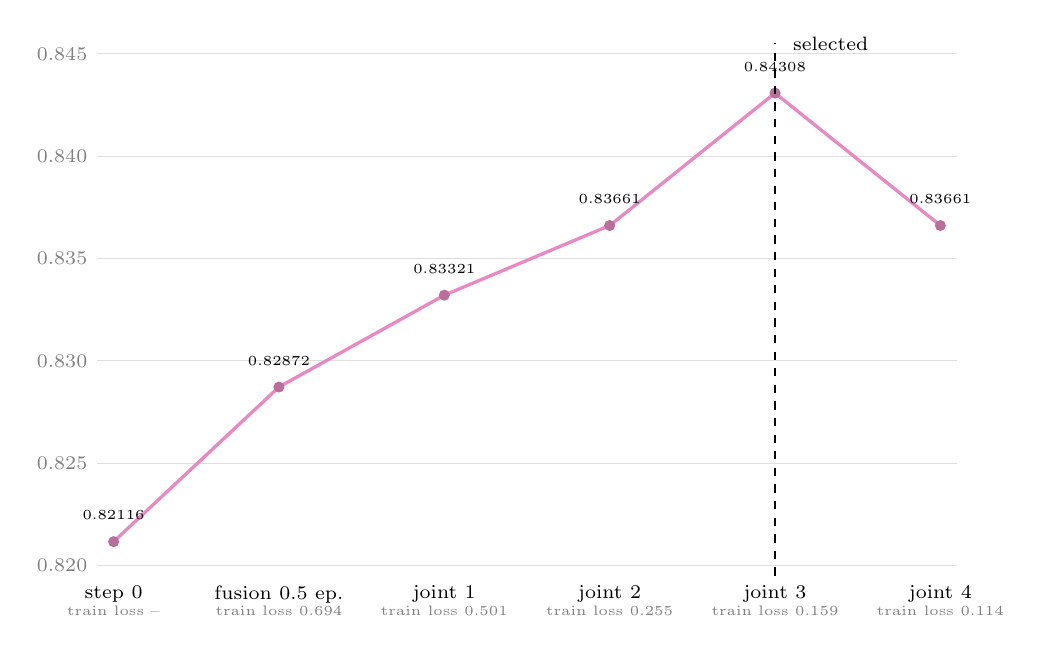
\begin{tikzpicture}[x=2.1cm,y=260cm]
  \foreach \t in {0.820,0.825,0.830,0.835,0.840,0.845} {
    \draw[gray!25] (-0.1,\t) -- (5.1,\t);
    \node[font=\scriptsize,gray,left] at (-0.1,\t) {\t};
  }
  \foreach \i/\name in {0/{step 0},1/{fusion 0.5 ep.},2/{joint 1},3/{joint 2},4/{joint 3},5/{joint 4}} {
    \node[font=\scriptsize,below] at (\i,0.8195) {\name};
  }
  \draw[mixc,very thick] (0,0.82116) -- (1,0.82872) -- (2,0.83321) -- (3,0.83661) -- (4,0.84308) -- (5,0.83661);
  \foreach \i/\v/\tl in {0/0.82116/{--},1/0.82872/0.694,2/0.83321/0.501,3/0.83661/0.255,4/0.84308/0.159,5/0.83661/0.114} {
    \fill[mixc!80!black] (\i,\v) circle (2pt);
    \node[font=\tiny,above] at (\i,\v+0.0006) {\v};
    \node[font=\tiny,gray] at (\i,0.8178) {train loss \tl};
  }
  \draw[black,dashed] (4,0.8195) -- (4,0.8455); \node[font=\scriptsize,anchor=west] at (4.05,0.8455) {selected};
\end{tikzpicture}
\caption{Training trajectory of the mixed model: macro F1 on prompt-test after each stage. The fourth joint epoch lowers the score while the training loss keeps falling, so the third is kept.}
\label{fig:trajectory}
\end{figure}

\begin{table}[ht]
\centering
\caption{Phase-three models on prompt-test (used for checkpoint selection, hence optimistic) and on public dev. Per-dimension values of the final-abt + DINO-only ensemble were recomputed from saved probabilities. The teacher is a per-dimension combination chosen on prompt-test and is used only to build distillation targets.}
\resizebox{\textwidth}{!}{\begin{tabular}{lrrrrrrrr}\toprule
Model & Macro F1 & Subject & Backgr. & Persp. & Indiv. & Text cl. & Text lang. & Public dev \\\midrule
SigLIP~2 + VQ (final-abt) & 0.821 & 0.846 & 0.881 & 0.755 & 0.959 & 0.766 & 0.720 & 0.832 \\
DINO-only, 81 tokens & 0.808 & 0.772 & 0.847 & 0.783 & 0.944 & 0.719 & 0.781 & -- \\
\textbf{Mixed (delivered)} & \textbf{0.843} & 0.868 & 0.875 & 0.776 & 0.970 & 0.769 & 0.798 & \textbf{0.842} \\\midrule
final-abt + DINO-only, 50/50 & 0.850 & 0.839 & 0.899 & 0.823 & 0.965 & 0.769 & 0.803 & 0.847 \\
Mixed + DINO-only, 50/50 & 0.856 & 0.841 & 0.897 & 0.833 & 0.970 & 0.776 & 0.819 & -- \\
Teacher (subject from mixed) & 0.860 & 0.868 & 0.897 & 0.833 & 0.970 & 0.776 & 0.819 & -- \\\bottomrule
\end{tabular}}
\label{tab:phase3}
\end{table}

On public dev the mixed model gains 0.010 over final-abt at the same decoder cost per token (Table~\ref{tab:phase3}). On prompt-test its gain over final-abt (+0.021, paired 95\% interval [0.006, 0.038]) exceeds the resolution of the split, and public dev confirms it. The prompt-test figure is somewhat larger, which is what we would expect when the epoch is chosen on the same set. Adding the DINO-only probabilities on top of the mixed model still helps perspective (0.776 to 0.833) but hurts subject, which is why we built a per-dimension teacher. We did not run a matched control that trains final-abt for the same epochs without DINOv3, so part of the gain may come from additional training of the other components.

\paragraph{Distillation (designed, not executed).} To transfer the ensemble's advantage into one decoder, we built soft teacher targets on the unlabelled public dev images, which the rules allow. Cells are masked by the scoring rules and by a per-dimension confidence threshold at which the teacher's precision on prompt-test is at least 0.90; this keeps 59\% of perspective cells and 76--93\% of the others. The pilot compares a distillation branch (masked soft cross-entropy at weight 0.5) with a supervised control trained for the same number of updates, and promotes the student only if macro F1 gains at least 0.008 with positive bootstrap lower bounds and at least 90\% of the original throughput. The code passes its CPU tests. At the time of writing, however, the pilot has not been run on a GPU, so we report no result.

\paragraph{Label-error search (negative result).} We flagged training cells where at least two models that had not seen the product confidently agreed on a different class. Of 57 candidates, visual inspection of the most extreme case per dimension found no certain error in six cases: four human labels were correct and two were ambiguous. In these cases, confident disagreement among models reflects blind spots the models share, not label noise. We did not submit the list.

\section{Efficient inference}
\label{sec:inference}
Speed and resource use account for a fifth of the challenge assessment \cite{challenge}, so we deliver one decoder and optimise its path from image to CSV (Table~\ref{tab:inference}). The original export of the mixed model ran at 5.98 images/s on dev on an H200, with the VQ tokenizer as the bottleneck (84 of 192 seconds on prompt-test). The \emph{fast path} merges LoRA into the decoder weights, sorts images by VQ grid size so the tokenizer can batch same-sized images, decodes images in a thread pool and runs OCR in its own thread one batch ahead. It agrees with the original export on 99.5--99.9\% of predictions per dimension on dev.

Switching the fp32 components (VQ tokenizer, SigLIP~2 and OCR) to \emph{TF32} matrix multiplication cut the VQ stage from 84 to 18 seconds on prompt-test. OCR then became the critical path. TF32 changes 0.7--0.9\% of VQ tokens, so only about a fifth of the images keep identical codes, yet macro F1 moves by only $-0.0008$. \emph{Selective perspective test-time augmentation} mirrors an image only when its two most likely perspective classes form a left/right pair with a margin below 0.15, a threshold fixed before evaluation. It averages the mirrored perspective distribution, with left and right swapped, into the original, while the other five dimensions come from the original view. On prompt-test it fires on 3.1\% of images and improves macro F1 by 0.0017 (95\% CI [0.0001, 0.0039]). Mirroring every image gives a similar point estimate (+0.0019, CI [$-0.0031$, 0.0071]) at 55\% of the speed. The full delivery configuration runs at 11.68 images/s on one H200 with 29~GiB peak memory, mirroring 4.0\% of dev images (Figure~\ref{fig:inference}).

\begin{figure}[ht]
\centering
\maybefigure{figures/inference-pipeline.png}{\textwidth}
\caption{Delivery inference path. Images are decoded in a thread pool and sorted by VQ grid size; OCR runs in a parallel thread one batch ahead; the fp32 components (VQ tokenizer, SigLIP~2, OCR) use TF32 and DINOv3 runs in bf16; the decoder runs with merged LoRA. Only images whose top two perspective classes are a close left/right pair are mirrored and re-scored.}
\label{fig:inference}
\end{figure}

\begin{table}[ht]
\centering
\caption{Inference ladder of the mixed model, from image to CSV with model loading excluded. GPU and batch size differ between rows; the 14.34 images/s row was measured on an H100 because H200s were unavailable. The TTA gain was measured without TF32.}
\resizebox{\textwidth}{!}{\begin{tabular}{llrrrl}\toprule
Configuration & GPU, batch & Dev img/s & Peak memory & Prompt-test F1 & Agreement with original \\\midrule
Original export & H200, 16 & 5.98 & 47~GiB & 0.8428 & reference \\
Fast path & H200, 32 & 8.53 & 79--88~GiB & 0.8432 & 99.5--99.9\% \\
Fast path + TF32 & H100, 16 & 14.34 & 23~GiB & 0.8424 & 99.1--100\% \\
Fast + TF32 + selective TTA (delivery) & H200, 32 & 11.68 & 29~GiB & -- & 97.5\% persp.; $\geq$99.4\% others \\\bottomrule
\end{tabular}}
\label{tab:inference}
\end{table}

At 11.68 images/s, 100,000 images need about 2.4 H200 GPU-hours, roughly \$12 at the \$5/h rate we used for estimates. The figure excludes model loading (76 seconds) and data transfer, and it is not an invoice. For comparison, the 70B zero-shot v2 protocol ran at 2.8 images/s on a shared gateway, and our earlier single-encoder model final-abt at 6.9 images/s on an H200. Extrapolating, the 5,292 final images would take about eight minutes at this rate. The public dev score of 0.842 came from the original export path. The delivery path agrees with it on at least 99.4\% of predictions outside perspective and 97.5\% for perspective, but it has no public score of its own.

\section{Discussion and limitations}
Prompt design and task-specific training both moved performance a long way, from 0.229 with an unsuitable zero-shot prompt to 0.842 on public dev for a trained 8B model with two frozen image encoders. Continuous encoders appear to complement Apertus' discrete tokens. The SigLIP branch started below LoRA + heads and overtook it only once OCR, spatial readouts and more data were added, and DINOv3 added 0.010 on public dev. We did not compare either encoder with a matched VQ-only or SigLIP-only control trained for the same budget.

Mean-pooled readouts are blind to mirroring by construction. In both branches, large perspective gains came with the addition of spatial differences and position-aware pooling, although other settings changed at the same time. Selective mirroring at inference adds a small gain whose confidence interval excludes zero.

The dataset exploration shaped the protocol as much as the model. With classes of 21 to 60 labelled examples in the whole dataset (F1), no local split can measure small gains on rare classes. We handled this with a two-signal protocol. A fixed, product-disjoint split, quantified by bootstrap intervals, serves for diagnostics and checkpoint choice, and the public leaderboard decides between models. The protocol leaves unconfirmed the gains of up to 0.026 that did not carry over and confirms the one that did. The context fields alone reach 0.438, so the image and the OCR text account for the large gap to the delivered model's 0.843.

Other limitations remain. Most runs use a single seed, and several changes were made together in every phase. Per-class scores of the rarest classes (Dutch, Italian, seals) rest on four to six prompt-test examples, and the delivered model's prompt-test score includes the choice of its epoch. The combined delivery configuration has no labelled score of its own. Finally, we have not demonstrated an offline, on-premise deployment, although every runtime component is open-weights and runs locally. The distillation pilot remains the most direct route to recover the ensemble's extra 0.005 in a single decoder. A last step follows from F1: once the model and its epoch are chosen, the held-out images can return to training. A final fit of the mixed model on all 11,876 labelled images (phase four) was being trained at the time of writing; by the protocol, it replaces the delivered model only if public dev confirms a gain beyond the leaderboard's resolution.

\section{Conclusion}
Apertus 1.5 8B can be turned into a competitive product-image classifier. Our model keeps its native VQ tokens and fuses frozen SigLIP~2 and DINOv3 features into 49 soft tokens. OCR text goes into the prompt, and six heads with spatially aware readouts are trained through LoRA. The delivered model reaches 0.842 macro F1 on public dev, between the organisers' Gemini Flash and Qwen references, and classifies 11.7 images per second on one GPU.

\section*{Code availability}
Code, configurations, the dataset analyses and the delivered model weights are available at \url{https://github.com/nathan-bymo/bymo-hack}.

\begin{thebibliography}{99}
\sloppy
\bibitem{apertus} Swiss AI, \emph{Apertus 1.5 Technical Report}, \url{https://arxiv.org/abs/2610.15542}.
\bibitem{siglip2} M.~Tschannen et al., \emph{SigLIP 2: Multilingual Vision-Language Encoders with Improved Semantic Understanding, Localization, and Dense Features}, arXiv:2502.14786, 2025.
\bibitem{dinov3} O.~Sim\'eoni et al., \emph{DINOv3}, arXiv:2508.10104, 2025.
\bibitem{lora_paper} E.~J.~Hu et al., \emph{LoRA: Low-Rank Adaptation of Large Language Models}, arXiv:2106.09685, 2021.
\bibitem{focal} T.-Y.~Lin et al., \emph{Focal Loss for Dense Object Detection}, ICCV 2017, arXiv:1708.02002.
\bibitem{cbloss} Y.~Cui et al., \emph{Class-Balanced Loss Based on Effective Number of Samples}, CVPR 2019, arXiv:1901.05555.
\bibitem{parseq} D.~Bautista and R.~Atienza, \emph{Scene Text Recognition with Permuted Autoregressive Sequence Models}, ECCV 2022, arXiv:2207.06966.
\bibitem{doctr} Mindee, \emph{docTR: Document Text Recognition}, \url{https://github.com/mindee/doctr}.
\bibitem{challenge} Challenge description, \url{https://github.com/nathan-bymo/bymo-hack/blob/main/challenge_description.md}.
\end{thebibliography}
\end{document}
